%!TEX root = ../report.tex

\section{Beweglichkeit}

Definition Beweglichkeit: Beweglichkeit ist die motorische Fähigkeit, Bewegungen willkürlich mit der erforderlichen Schwingungsweite ausführen zu können.

Verwandte Begriffe: \textbf{Gelenkigkeit} = Schwingungsweite von Gelenken, \textbf{Dehnfähigkeit} = Dehnbarkeit von Muskeln und Sehnen

Optimalitätseigenschaft: Stabilität versus Mobilität, Hypo- versus Hypermobilität

\subsection{Systematik und Determinanten}

\subsubsection*{Dimensionen }

\begin{itemize}
    \item Passive Beweglichkeit: Beweglichkeit die unter Einwirken einer externen Kraft erreicht wird (z.B. Spagat, Schwerkraft)
    Aktive Beweglichkeit: Beweglichkeit, die durch aktive Muskelarbeit erreicht wird (z.B. Armschwung, Schuss, Spagatsprung)
\end{itemize}

Methoden im Beweglichkeitstraining:
\begin{itemize}
    \item aktiv: Antagonisten bewirken Dehnung
    \item passiv: Partner, Schwerkraft, andere Muskeln bewirken Dehnung
    \item statisch: langsames Einnehmen der Dehnposition, ohne Auslösung des Muskelreflexes (intensiv)
    \item dynamisch: schnelles, federndes Einnehmen der Dehnposition, mit (unter Inkaufnahme der) Auslösung des Muskelreflexes
\end{itemize}

\subsubsection*{Muskelreflex}

Schnelle Bewegungen lösen den Muskelreflex aus, aber das Auslösen des Muskelreflexes ist kontraproduktiv zur Absicht der Dehnung. Wenn die Dehnung intensiv sein soll, sollte Muskelreflex nicht (nur minimal) ausgelöst werden, d.h. keine schnellen Bewegungen.

Der Muskeltonus ist Ausdruck des systemischen Erregungszustandes. Zu hoch impliziert sanfte Dehnung und Entspannungsübungen, zu niedrig dagegen intensive Dehnung.

\subsubsection*{Determinanten}

Allgemein:
Ein Gelenk besteht aus Muskeln und Sehnen, Knochen, Knorpel und der Gelenkkapsel mit Bändern.
Es gibt verschiedene Rezeptoren:
\begin{itemize}
    \item Ruffini-Körperchen sind Mechanorezeptoren in Kapsel und Haut und reagieren auf Druck und Dehnung. Dabei registrieren sie das Ausmaß und die Geschwindigkeit von Gelenkbewegungen.
    \item Vater-Pacini-Körperchen sind Mechanorezeptoren im Gelenkbindegewebe und registrieren Beschleunigungen.
    \item Golgi-Sehnenorgan sitzt im Übergang zwischen Muskeln und Sehnen und registriert dort die Muskelspannung. Unter Umständen gibt es eine Reflexantwort.
    \item Muskelspindeln sind quergestreifte Muskelfasern, die ebenfalls als Mechanorezeptoren dienen. Sie lösen den Eigenreflex aus und messen das Ausmaß und die Geschwindigkeit einer Muskelbewegung.
\end{itemize}

\begin{minipage}{0.4\textwidth}
Entscheidend sind folgende anatomische Eigenschaften:
\begin{itemize}
    \item Freiheitsgrade und Funktionstüchtigkeit der Gelenke
    \item Bandhafte- und kapsuläre Hemmung
    \item Titinfilamente (hauptsächlich verantwortlich für Widerstand)
    \item Tendo-muskuläre Reflexschaltungen (Hemmungen)
\end{itemize}
\end{minipage}
\begin{minipage}{0.6\textwidth}
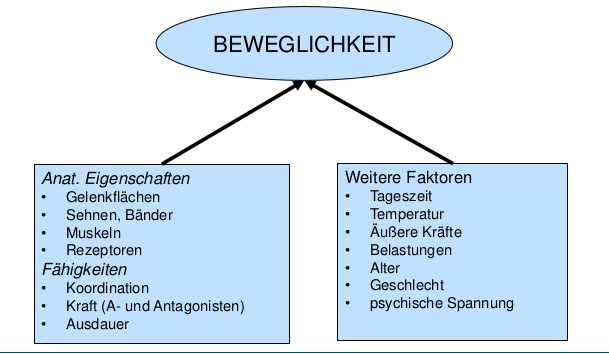
\includegraphics[width=\textwidth]{pictures/beweg_determinanten}
\end{minipage}
Weitere Einflussfaktoren:
\begin{itemize}
    \item Alter: Abnahme der Elastizität (H 2 O-Verlust; Weniger Zellen)
    \item Geschlecht: Einfluss des Östrogens
    \item Ausdauer: Kein Beweglichkeitstraining im Ermüdungszustand
\end{itemize}

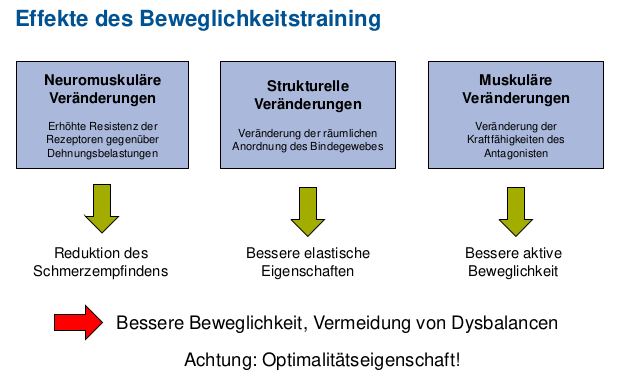
\includegraphics[width=0.9\textwidth]{pictures/beweg_effekte}
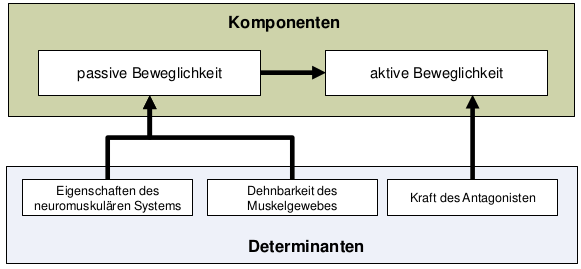
\includegraphics[width=0.9\textwidth]{pictures/beweg_determinanten2}

\subsection{Bedeutung}

Beweglichkeit kann Bestandteil von Wettkampfleistungen sein (Bsp: bessere Bepunktung von Spagat in der Gymnastik) oder Voraussetzung für Wettkampfleistungen, konditionelle Fähigkeiten oder Teilleistungen sein (Bsp: bessere performance von beweglicheren Fußballspielern).

Als Beweglichkeitsreserve bezeichnet man die Differenz zwischen erforderlichem und maximalem Bewegungsausschlag. Eine große Reserve ist erstrebsam, weil dann nicht bis an die Dehnbarkeitsgrenze belastet werden muss (Ökonomisierung) und die Bewegung unter geringerem Widerstand ablaufen kann. Auch im Fitness- und Gesundheitstraining ist Dehnen zur Vermeidung von Dysbalancen und Verkürzungen relevant.

\subsubsection*{Aufwärmen vs Dehntraining}

Seit Mitte der 90er Jahren ist bekannt, dass intensives statisches Dehnen (Stretching) in der Aufwärmphase genau das Gegenteil von dem, was man sich erhofft, bewirkt.
Statt leistungssteigernd und verletzungsmindern zu wirken, führt es zu geringerer Leistung und einem größerem Verletzungsrisiko. Ausmaß: 4-8\% weniger vertikale Sprungleistung und 5-10\% Reaktivkraftleistungen

Gründe:
\begin{itemize}
    \item Geringere Kraftproduktion Muskel-Sehnen-Komplex (Verlängerung, Belastung der fibrillären Strukturen)
    \item Periphere neuromuskuläre Veränderungen, z.B. Reduktion der
    \item Erregbarkeit der Motoneurone
    \item Zentrale psychophysiologische Desaktivierungsprozesse, Senkung der zentralen Aktivierung
\end{itemize}

\subsection{Diagnostik}
